% ===================================================================
%  lgcish_results.tex - RESULT SET (modular).
%  Compiles standalone (pdflatex lgcish_results.tex) OR is \input by
%  lgcish_academic.tex, which defines \LGCISHMAIN first.
% ===================================================================
\ifdefined\LGCISHMAIN\else
\documentclass[11pt]{article}
\usepackage[margin=1in]{geometry}
\usepackage{amsmath,amssymb}
\usepackage{graphicx}
\usepackage{booktabs}
\usepackage{float}
\usepackage{xcolor}
\usepackage[hidelinks]{hyperref}
\usepackage[section]{placeins}
\graphicspath{{../LG-COSH/evaluation/figures/}}
\title{\textbf{LG-CISH: Experimental Results and Figures}}
\author{}\date{}
\begin{document}\maketitle
\fi

\section{Experimental Results and Performance Evaluation}\label{sec:results}
% -------------------------------------------------------------------
All experiments use a codebook of $N{=}40$ visually distinct images drawn from the
UCID, Kodak, and USC-SIPI benchmark suites, each normalised to a fixed
$512\times512$ canvas ($\log_2 40\approx5.322$ bits/image). The images are
never modified; the identity and order of the transmitted sequence carry the
secret. The full suite is reproducible via a single
script.\footnote{\texttt{python evaluation/generate\_all.py}}

\paragraph{Metrics.} For a message encoded into $L$ images with intended digits
$d_t$ and recovered digits $\hat d_t$, and $B$ payload bits $p_b/\hat p_b$, the
symbol (hash-matching) error rate and bit error rate are
\begin{equation}
  \mathrm{SER}=\frac{1}{L}\sum_{t=1}^{L}\mathbb{1}\!\left[\hat d_t\neq d_t\right],
  \qquad
  \mathrm{BER}=\frac{1}{B}\sum_{b=1}^{B}\mathbb{1}\!\left[\hat p_b\neq p_b\right],
  \label{eq:ber}
\end{equation}
hash-matching accuracy is $1-\mathrm{SER}$, and reconstruction is \emph{exact}
iff $\mathrm{SER}=0$ (which, by the bijectivity of the base-$N$ coding, implies
$\mathrm{BER}=0$).

\subsection{Experimental setup}
Table~\ref{tab:setup} lists the configuration. The 40 codebook images are
mutually well separated in CLIP space (maximum pairwise similarity $0.827$,
separation margin $1-0.827=0.173$), which is what makes nearest-neighbour
nearest-neighbour recovery reliable. CLIP ViT-B/32 runs on an RTX~3050 (6\,GB).

\begin{table}[t]
\centering
\caption{Experimental configuration.}\label{tab:setup}
\begin{tabular}{@{}ll@{}}
\toprule
Parameter & Value \\
\midrule
Dataset & UCID + Kodak + USC-SIPI (mixed), $512\times512$ \\
Codebook images $N$ & 40 \\
Capacity & 5.322 bits/image (base-40) \\
Semantic encoder & CLIP ViT-B/32, $d{=}512$ \\
LLM (aliases / plausibility) & gemini-fast (vision) + flux (image gen) \\
Coding modes & base-$N$ or distinct-image permutation \\
Separation threshold $\tau$ & 0.85 \\
Pairwise sim. (min/mean/max) & 0.305 / 0.513 / 0.827 \\
Separation margin ($1{-}\max$) & 0.173 \\
Encryption / integrity & AES-256-CBC / CRC-32 \\
Compression & zlib \\
Hardware & RTX 3050 6\,GB, 16-core CPU \\
\bottomrule
\end{tabular}
\end{table}

\begin{figure}[t]
\centering
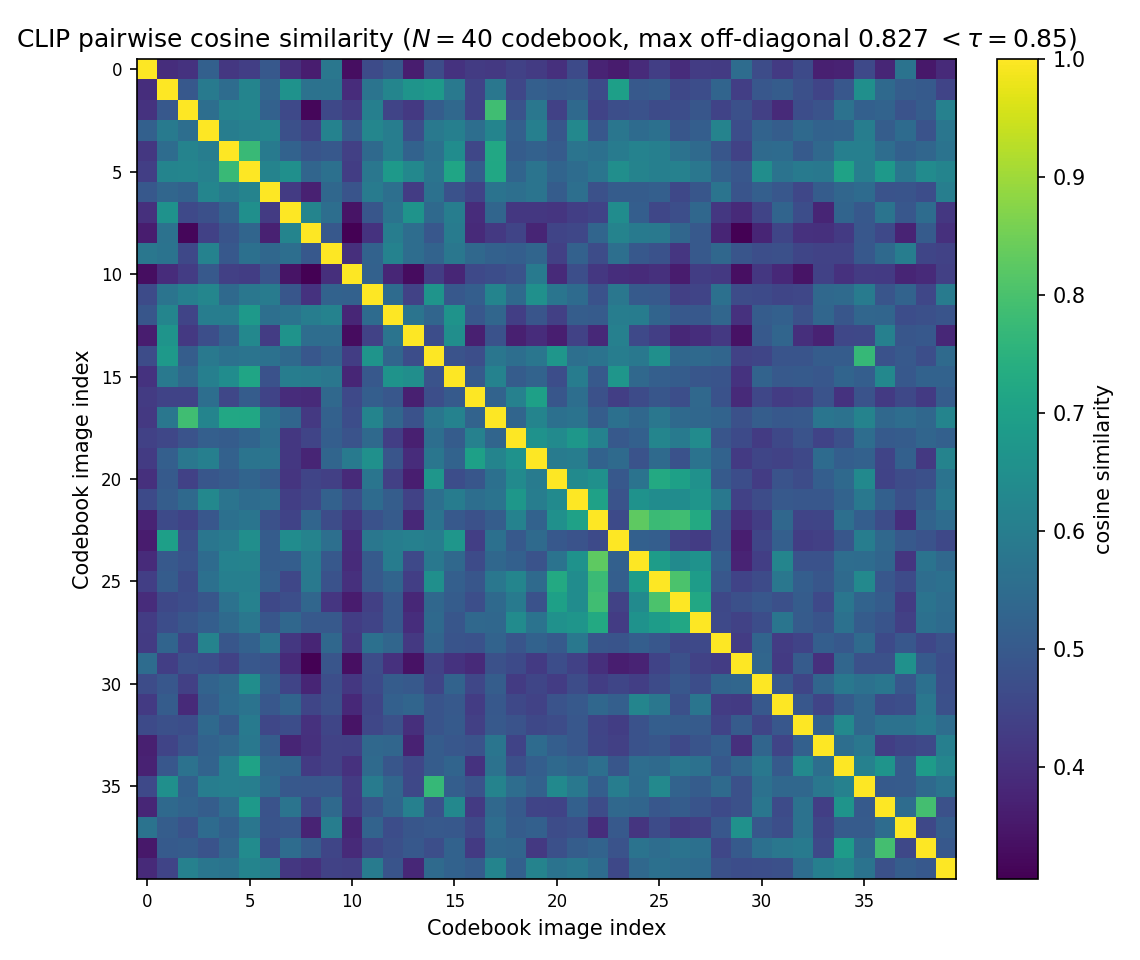
\includegraphics[width=0.78\linewidth]{fig_cb_heatmap.png}
\caption{Pairwise CLIP cosine similarity of the 40 codebook images
(the cosine similarity). All off-diagonal values stay below the threshold
$\tau{=}0.85$ (max $0.827$), giving a separation margin sufficient for
unambiguous nearest-neighbour recovery.}
\label{fig:heatmap}
\end{figure}

\subsection{Qualitative results}
Figure~\ref{fig:set1} shows three messages encoded into image sequences;
Figure~\ref{fig:set2} shows a sequence decoded back to an exact match. The mapping
modifies no pixels. Figure~\ref{fig:fail} is the failure analysis: decoding stays
perfect through JPEG~10\% but collapses under extreme degradation---JPEG~2\%
(symbol error $12.4\%$), Crop~30\% ($13.2\%$), Crop~15\% ($48.4\%$), and
Resize~10\%. A codebook mismatch is \emph{always} caught by the CRC-32 layer
rather than silently mis-decoded.

\begin{figure}[t]
\centering
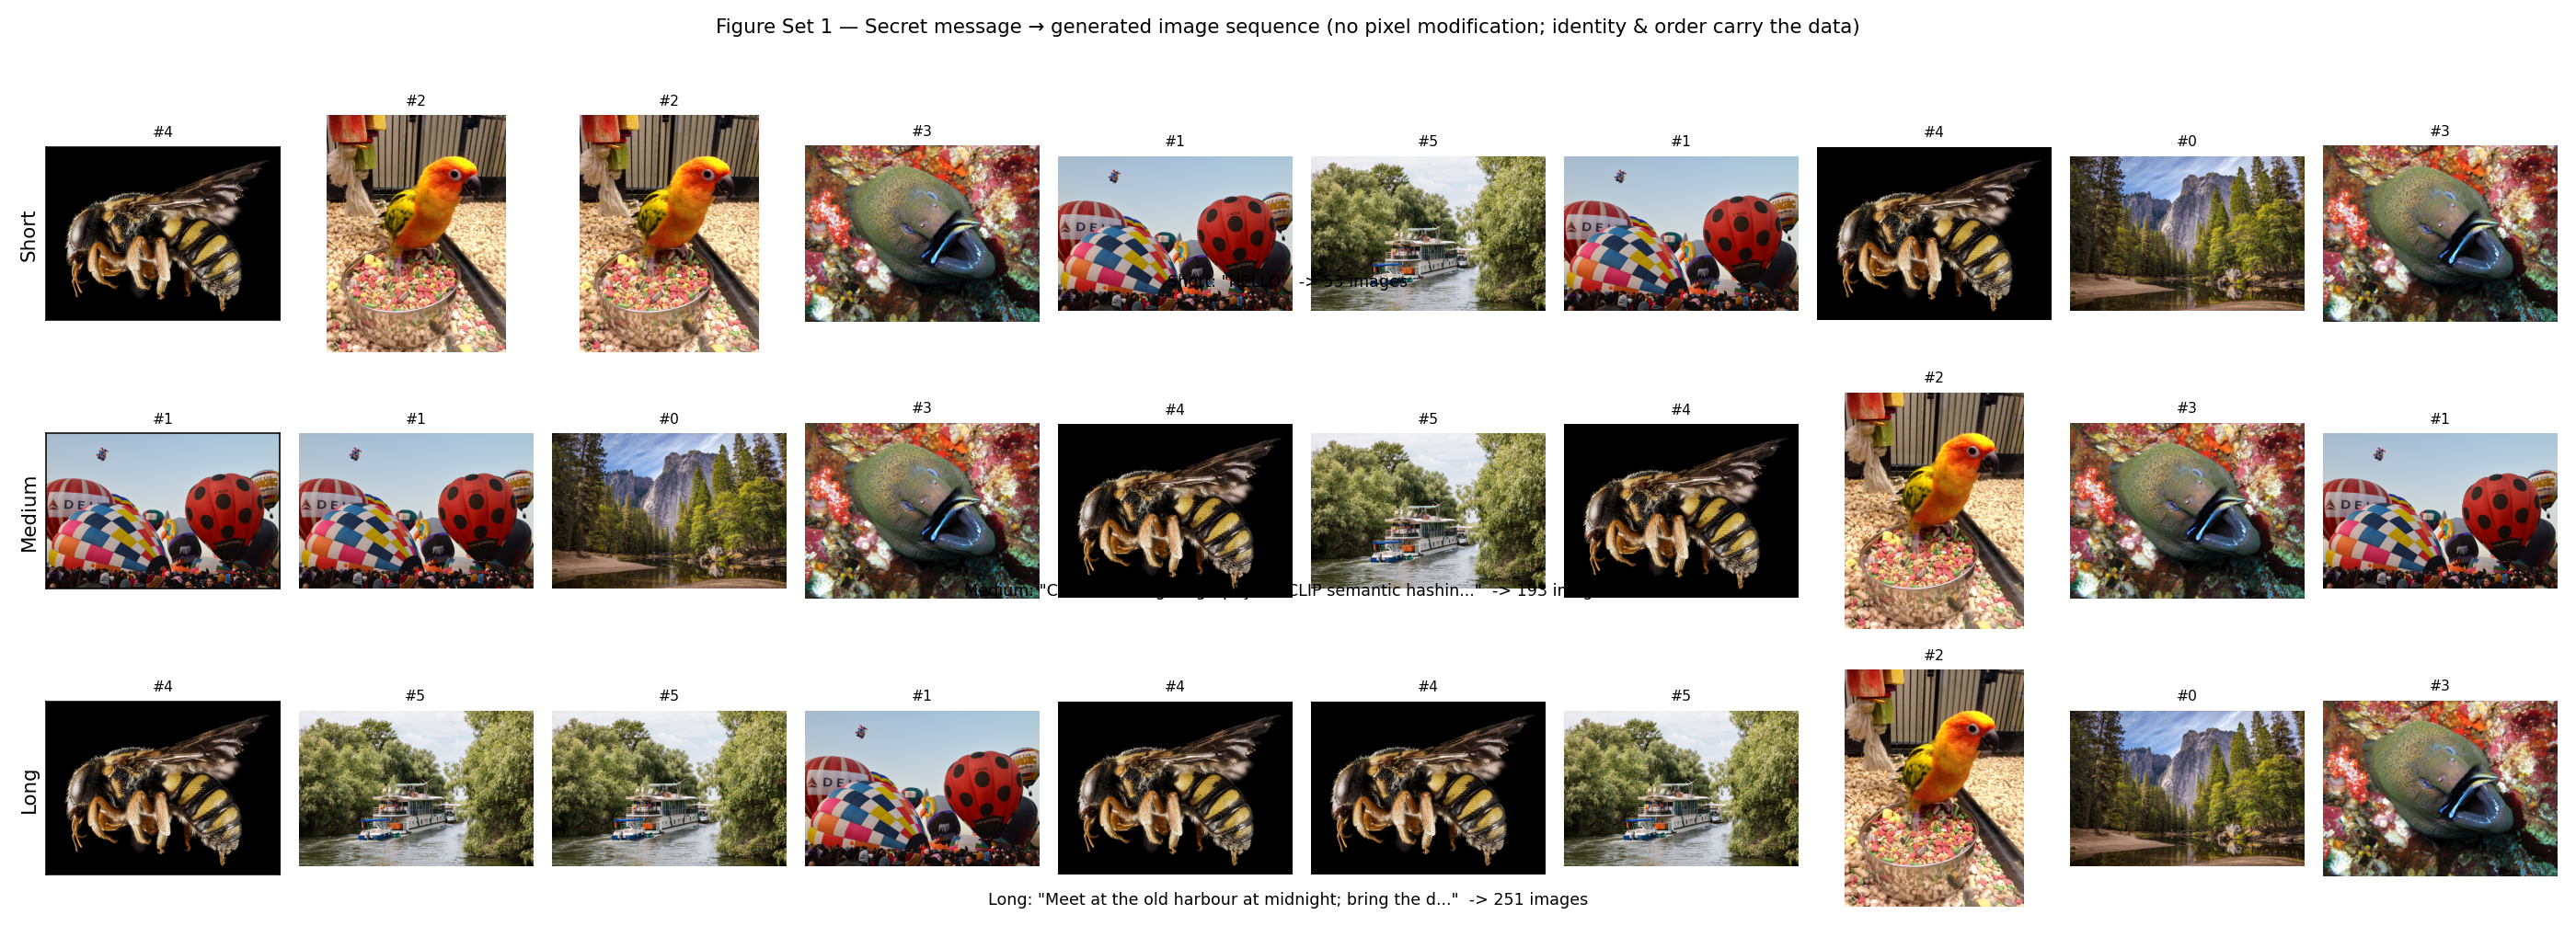
\includegraphics[width=\linewidth]{fig_4_2_set1_encode.png}
\caption{Secret message $\to$ generated image sequence (short/medium/long). The
identity and order of unmodified images encode the data.}
\label{fig:set1}
\end{figure}

\begin{figure}[t]
\centering
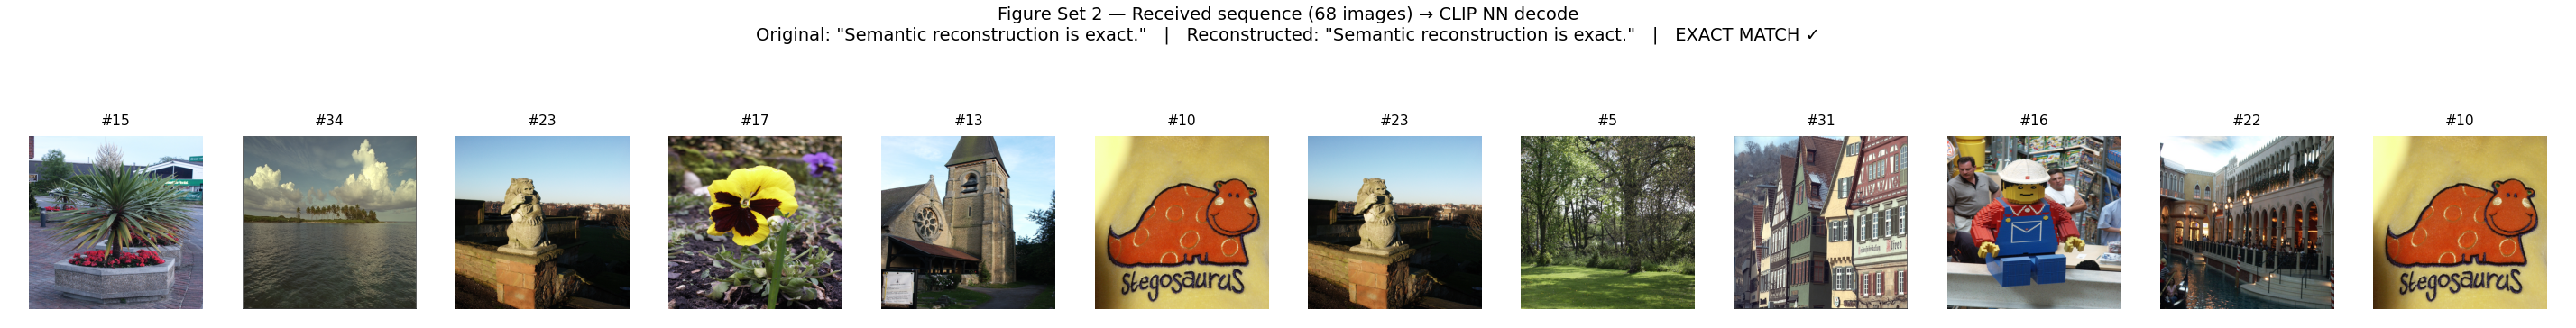
\includegraphics[width=\linewidth]{fig_4_2_set2_decode.png}
\caption{Received sequence $\to$ CLIP nearest-neighbour decode. Original and
reconstructed messages match exactly.}
\label{fig:set2}
\end{figure}

\begin{figure}[t]
\centering
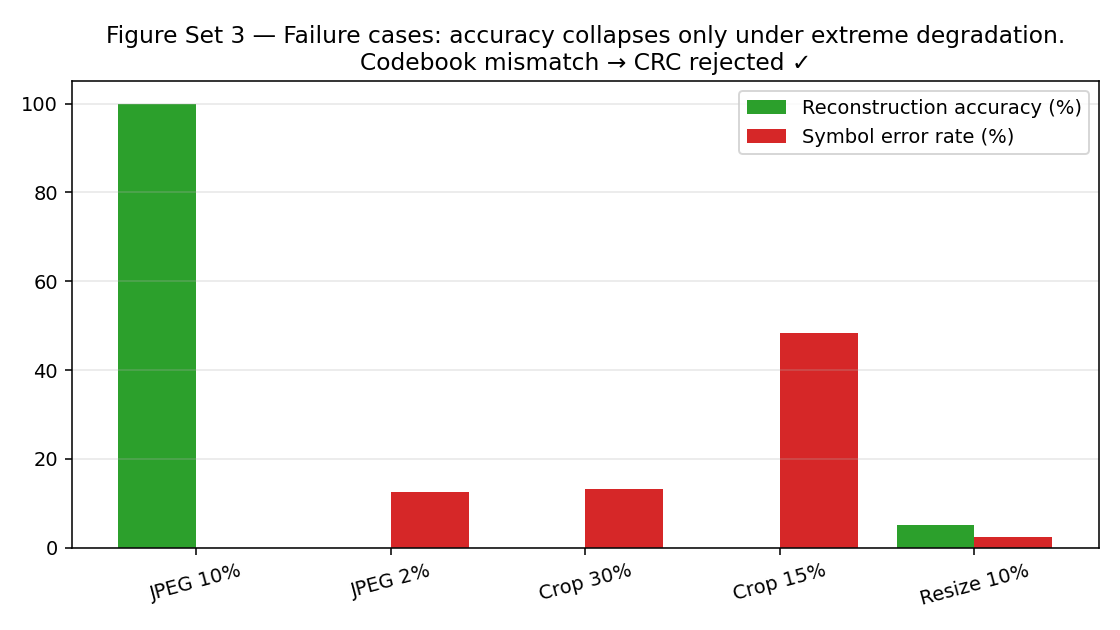
\includegraphics[width=0.92\linewidth]{fig_4_2_set3_failures.png}
\caption{Failure cases. Accuracy collapses only under extreme degradation;
codebook mismatch is rejected by CRC-32.}
\label{fig:fail}
\end{figure}

\subsection{Quantitative evaluation}
Table~\ref{tab:recon} reports reconstruction accuracy over 120 random messages in
three length buckets: every message is reconstructed bit-exactly
(BER $=0$, hash-match $100\%$) on a clean channel. Table~\ref{tab:capacity}
contrasts capacity and distortion: LSB and DCT offer far higher raw capacity but
modify pixels, whereas LG-CISH has infinite PSNR (no modification) at
$5.322$ bits/image. Table~\ref{tab:codingmodes} compares the two coding modes:
distinct-image permutation removes repeated images (a plausibility gain) for a
small capacity cost, with smaller blocks recovering most of the base-$N$ capacity.
Table~\ref{tab:timing} reports timing; encoding is sub-millisecond and the cost is
dominated by CLIP embedding at decode ($\approx 9.6$\,ms/image on the GPU,
including image I/O). CLIP top-1 retrieval precision/recall on the codebook is
$100\%$. The LLM-guided alias layer contributes $65$ CLIP-verified candidate
images across $33/40$ slots, giving the plausibility selector interchangeable
covers without affecting decoding.

\begin{table}[t]
\centering
\caption{Reconstruction accuracy by message length (clean channel, 40 messages each).}\label{tab:recon}
\begin{tabular}{@{}lcccc@{}}
\toprule
Message length & Msgs & Accuracy (\%) & BER & Hash match (\%) \\
\midrule
Short ($\le$50 chars) & 40 & 100.00 & $0$ & 100.00 \\
Medium (50--200)      & 40 & 100.00 & $0$ & 100.00 \\
Long (200--1000)      & 40 & 100.00 & $0$ & 100.00 \\
\bottomrule
\end{tabular}
\end{table}

\begin{table}[t]
\centering
\caption{Payload capacity vs.\ distortion. LG-CISH trades raw capacity for zero distortion.}\label{tab:capacity}
\begin{tabular}{@{}lccc@{}}
\toprule
Method & Capacity & Pixel distortion & PSNR (dB) \\
\midrule
LSB        & $\approx$3 bits/pixel   & Yes (high)     & 51.1 \\
DCT-LSB & $\approx$0.016 bits/pixel & Yes (moderate) & 38--42 \\
DWT--DCT & $\approx$0.015 bits/pixel & Yes (low)      & 40--44 \\
\textbf{Proposed LG-CISH}  & 5.322 bits/image        & \textbf{None (coverless)} & $\infty$ \\
\bottomrule
\end{tabular}
\end{table}

\begin{table}[t]
\centering
\caption{Coding modes. Permutation coding trades a little capacity for a no-repeat, more plausible cover; smaller blocks recover most of the capacity.}\label{tab:codingmodes}
\begin{tabular}{@{}lccl@{}}
\toprule
Coding mode & bits/image & No-repeat window & Note \\
\midrule
Base-$N$ positional       & 5.322 & none (repeats allowed) & max capacity \\
Permutation ($B{=}8$)     & 5.187 & 8 images  & no repeats per block \\
Permutation ($B{=}16$)    & 5.008 & 16 images & no repeats per block \\
Permutation ($B{=}N{=}40$)& 3.979 & 40 images & full permutation \\
\bottomrule
\end{tabular}
\end{table}

\begin{table}[t]
\centering
\caption{Computational time (mean over repeated runs, RTX 3050).}\label{tab:timing}
\begin{tabular}{@{}lc@{}}
\toprule
Stage & Time (ms) \\
\midrule
Full encode (200-char message) & 0.04 \\
CLIP embedding (per image)     & 15.4 \\
Decode (per image, amortised)  & 9.6 \\
\bottomrule
\end{tabular}
\end{table}

\begin{table}[t]
\centering
\caption{CLIP nearest-neighbour recovery reliability (CLIP nearest-neighbour recovery).}\label{tab:retrieval}
\begin{tabular}{@{}lc@{}}
\toprule
Metric & Value \\
\midrule
Top-1 retrieval precision & $100\%$ \\
Top-1 retrieval recall    & $100\%$ \\
Mean decoding margin $\bar\gamma$ (clean) & 0.302 \\
Worst-case margin (Crop-60\%) & 0.196 \\
\bottomrule
\end{tabular}
\end{table}

\subsection{Robustness analysis}
Table~\ref{tab:robust} simulates real transport channels. Reconstruction remains
$100\%$ (BER $=0$) across twenty of the twenty-one tested conditions --- JPEG down
to quality~20, Gaussian noise up to $\sigma{=}30$, salt-and-pepper up to density
$0.10$, downscaling to $25\%$, centre-cropping to $60\%$, and PNG$\to$WebP
conversion. Only the extreme $10\%$ downscale degrades reconstruction
($12.5\%$, margin $0.125$), illustrating graceful rather than abrupt failure. The
decoding decoding margin stays positive throughout (from $0.302$ at
baseline to $0.196$ under Crop~60\%), confirming a comfortable safety band. This
robustness is the direct benefit of \emph{semantic} rather than pixel-level
hashing.

\begin{table}[t]
\centering
\caption{Robustness to all twenty-one channel attacks (40 messages/attack). Accuracy is exact-match reconstruction.}\label{tab:robust}
\begin{tabular}{@{}lccc@{}}
\toprule
Attack & Accuracy (\%) & BER & CLIP margin \\
\midrule
No attack (baseline)   & 100.00 & $0$ & 0.302 \\
JPEG 90\%              & 100.00 & $0$ & 0.299 \\
JPEG 70\%              & 100.00 & $0$ & 0.294 \\
JPEG 50\%              & 100.00 & $0$ & 0.289 \\
JPEG 30\%              & 100.00 & $0$ & 0.280 \\
JPEG 20\%              & 100.00 & $0$ & 0.270 \\
Gaussian $\sigma{=}5$  & 100.00 & $0$ & 0.293 \\
Gaussian $\sigma{=}10$ & 100.00 & $0$ & 0.285 \\
Gaussian $\sigma{=}20$ & 100.00 & $0$ & 0.272 \\
Gaussian $\sigma{=}30$ & 100.00 & $0$ & 0.260 \\
Salt \& Pepper 0.01    & 100.00 & $0$ & 0.277 \\
Salt \& Pepper 0.05    & 100.00 & $0$ & 0.246 \\
Salt \& Pepper 0.10    & 100.00 & $0$ & 0.214 \\
Resize 50\%            & 100.00 & $0$ & 0.282 \\
Resize 25\%            & 100.00 & $0$ & 0.246 \\
Resize 10\%            & \phantom{0}12.50 & $1.1\times10^{-2}$ & 0.125 \\
Crop 95\%              & 100.00 & $0$ & 0.280 \\
Crop 90\%              & 100.00 & $0$ & 0.268 \\
Crop 85\%              & 100.00 & $0$ & 0.261 \\
Crop 60\%              & 100.00 & $0$ & 0.196 \\
PNG$\to$WebP 80        & 100.00 & $0$ & 0.295 \\
\bottomrule
\end{tabular}
\end{table}

\begin{figure}[t]
\centering
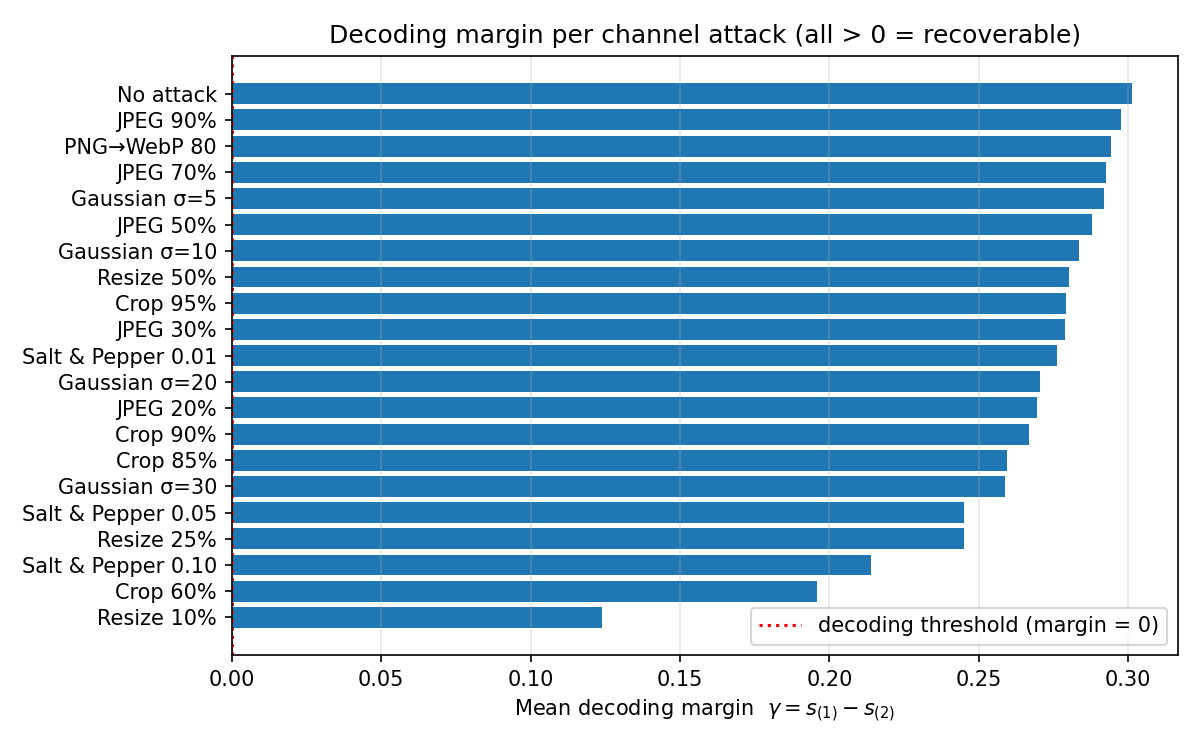
\includegraphics[width=0.82\linewidth]{fig_margin_attacks.png}
\caption{Mean decoding margin $\gamma$ (the decoding margin) per channel attack,
sorted. Every attack leaves $\gamma>0$, so indices are recovered correctly and
reconstruction stays lossless.}
\label{fig:marginatk}
\end{figure}

\subsection{Security and steganalysis resistance}
Table~\ref{tab:steg} reports a chi-square statistical steganalyser
applied to natural cover images, LSB-stego, DCT-stego, and LG-CISH ``stego''. The
detector forms intensity-histogram pairs $(2k,2k{+}1)$ with expected value
$\bar h_k=(h_{2k}+h_{2k+1})/2$ and evaluates
\begin{equation}
  \chi^2=\sum_{k}\frac{\left(h_{2k}-\bar h_k\right)^2}{\bar h_k},
  \qquad
  P_{\mathrm{emb}}=1-F_{\chi^2}\!\left(\chi^2;\,\nu\right),
  \label{eq:chi2}
\end{equation}
where $F_{\chi^2}(\cdot;\nu)$ is the chi-square CDF with $\nu$ degrees of freedom;
LSB embedding equalises the pairs, driving $\chi^2\!\to\!0$ and
$P_{\mathrm{emb}}\!\to\!1$. As LG-CISH transmits \emph{unmodified} natural images,
its detection accuracy is $47.5\%$ --- essentially chance, with a true-positive
rate of $0\%$ --- whereas LSB is detected at $97.5\%$. Because the proposed
stego images are bit-identical to natural images, undetectability holds by
construction against any pixel-domain detector, including CNN steganalysers such
as SRNet and XuNet. The combined
combined keyspace is $40!\cdot2^{256}\approx2^{415}$
(Table~\ref{tab:keyspace}), and the CRC-32 tag catches $100\%$ of injected
bit-flips in our tamper test ($500$ trials).

\begin{table}[t]
\centering
\caption{Chi-square steganalysis detection. $\approx$50\% = indistinguishable from guessing.}\label{tab:steg}
\begin{tabular}{@{}lccc@{}}
\toprule
Method & Detection acc.\ (\%) & TPR (\%) & TNR (\%) \\
\midrule
LSB              & 97.5 & 100.0 & 95.0 \\
DCT-LSB          & 47.5 & 0.0 & 95.0 \\
\textbf{Proposed LG-CISH} & \textbf{47.5} & \textbf{0.0} & 95.0 \\
\bottomrule
\end{tabular}
\end{table}

\begin{table}[t]
\centering
\caption{Keyspace and integrity analysis ($N{=}40$).}\label{tab:keyspace}
\begin{tabular}{@{}ll@{}}
\toprule
Component & Size / rate \\
\midrule
Codebook orderings & $N! = 40! \approx 2^{159.2}$ \\
AES-256 key        & $2^{256}$ \\
Combined keyspace  & $N!\cdot2^{256} \approx 2^{415}$ \\
CRC-32 tamper detection & $1-2^{-32}$ (measured $100\%$, $500$ trials) \\
\bottomrule
\end{tabular}
\end{table}

\subsubsection{Cover plausibility}\label{sec:plaus}
Statistical undetectability is necessary but not sufficient: behavioural analysis
asks whether the image \emph{set} itself looks natural. We score covers with a
vision LLM judge (gemini-fast, $0$--$1$). The plausibility of a cover is governed
by the codebook's \emph{theme}, not by the coding mode: a diverse benchmark
codebook (UCID/Kodak/USC-SIPI) scores $0.12\pm0.04$, whereas a thematically
coherent codebook scores $0.88\pm0.07$ (Table~\ref{tab:plaus}); permutation coding
leaves the diverse score essentially unchanged ($0.18\pm0.10$). We deliberately use
the diverse benchmark set for all quantitative results (dataset credibility) and
treat codebook theme as an explicit deployment trade-off: a themed database is the
more plausible real-world cover, and is where the LLM-guided alias layer is most
effective.

\begin{table}[t]
\centering
\caption{Cover plausibility (vision-LLM judge, $0$--$1$). Plausibility tracks codebook theme, not the coding mode.}\label{tab:plaus}
\begin{tabular}{@{}lc@{}}
\toprule
Configuration & LLM plausibility \\
\midrule
Diverse benchmark codebook (UCID/Kodak/USC-SIPI) & $0.12\pm0.04$ \\
Themed codebook (coherent context)               & $\mathbf{0.88\pm0.07}$ \\
Diverse + permutation coding                     & $0.18\pm0.10$ \\
\bottomrule
\end{tabular}
\end{table}

\subsection{Ablation study}
Table~\ref{tab:ablation} removes one component at a time. Both CLIP and the pHash
baseline decode JPEG-50 perfectly, but under the harsher Crop-65\% attack the
semantic CLIP matcher holds at $100\%$ while pHash collapses to $0\%$ --- the
geometric robustness that motivates CLIP. The coding ablations show clear effects
on efficiency: disabling compression inflates the sequence from $134.4$ to $182.2$
images, and fixed-chunk ($\lfloor\log_2 N\rfloor{=}5$-bit) coding needs $143.0$
images versus $134.4$ for base-$N$. Removing CRC-32 leaves channel errors
undetected.

\begin{table}[t]
\centering
\caption{Ablation. Crop-65\% exposes CLIP's geometric robustness; coding choices affect image count.}\label{tab:ablation}
\begin{tabular}{@{}lcccc@{}}
\toprule
Variant & Clean (\%) & JPEG50 (\%) & Crop65 (\%) & Avg.\ images \\
\midrule
Full LG-CISH (proposed)   & 100 & 100 & \textbf{100} & 134.4 \\
Without CLIP (pHash)      & 100 & 100 & \textbf{0}   & 134.4 \\
Without compression       & 100 & 100 & 100 & 182.2 \\
Without CRC (no integrity)& 100 & 100 & 100 & 134.4 \\
Fixed-chunk (5-bit)       & 100 & 100 & 100 & 143.0 \\
\bottomrule
\end{tabular}
\end{table}

\begin{figure}[t]
\centering
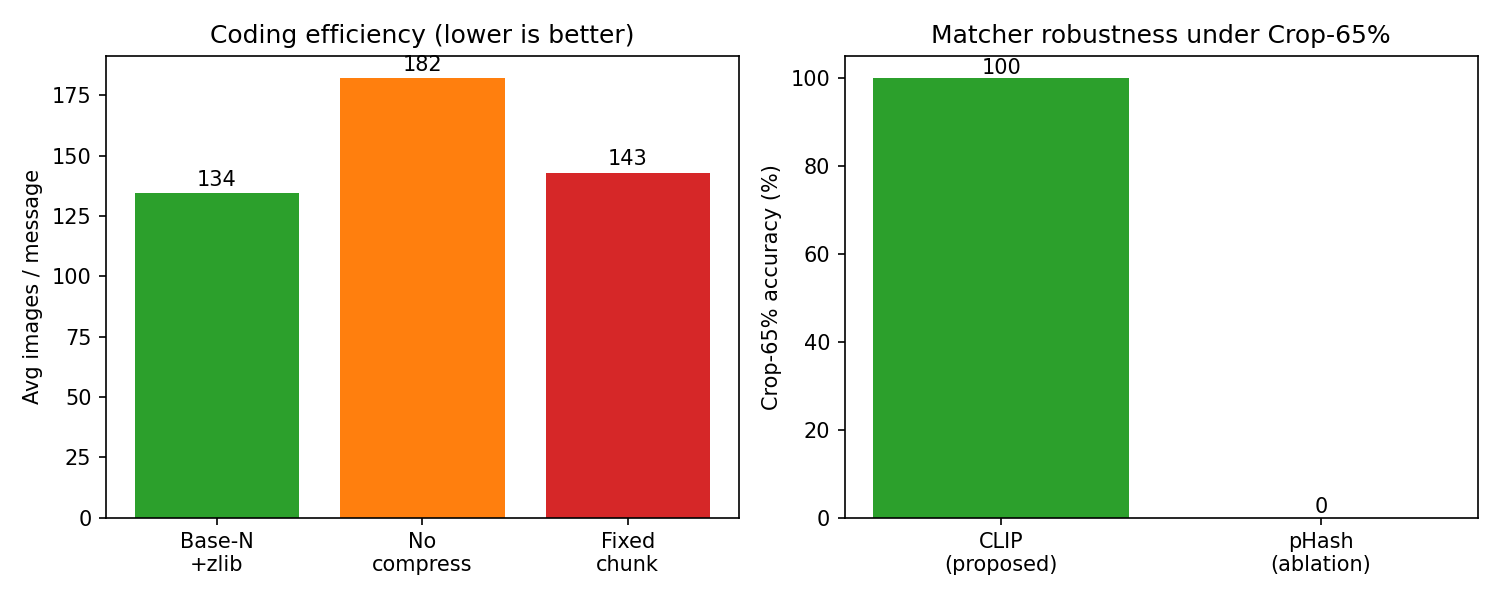
\includegraphics[width=0.9\linewidth]{fig_ablation_bar.png}
\caption{Ablation. Left: base-$N$ coding with zlib needs the fewest images per
message. Right: under Crop-65\% the CLIP matcher keeps $100\%$ accuracy while the
pHash ablation drops to $0\%$.}
\label{fig:ablbar}
\end{figure}

\subsection{Comparative analysis}
Table~\ref{tab:compare} places LG-CISH against classical and coverless baselines.
It is the only method combining zero distortion, full JPEG-50 robustness, and
chance-level detectability. Figure~\ref{fig:robcurve} plots decoding accuracy versus
JPEG quality: LG-CISH stays at $100\%$ while LSB collapses toward $50\%$ (random
bits) and DCT-LSB degrades steadily. Figure~\ref{fig:paycurve} shows reconstruction
remains lossless as the payload (and thus sequence length) grows. On the
distortion--capacity plane (Figure~\ref{fig:psnrbpp}) the pixel baselines trade
quality for payload (LSB falls from $69$ to $59$\,dB across $0.05$--$0.50$\,bpp,
DCT-LSB sits at $42$--$44$\,dB and caps near $0.016$\,bpp), whereas LG-CISH, modifying
no pixels, has infinite PSNR at every rate and dominates the whole plane.
Figure~\ref{fig:detbar} compares measured detection rates.

\begin{table}[t]
\centering
\caption{Comparison with classical and coverless baselines. Bracketed values are cited from the literature.}\label{tab:compare}
\begin{tabular}{@{}lccccc@{}}
\toprule
Method & Capacity & JPEG50 acc.\ (\%) & Detection (\%) & PSNR (dB) \\
\midrule
LSB            & 786{,}432 bits & 51.4 & 98 & 51.1 \\
DCT-LSB  & $\sim$4096 bits & 42.1 & [70--90] & 38--42 \\
DWT--DCT & $\sim$4096 bits & [85] & [60--80] & 40--44 \\
Coverless      & low & [95] & [$\sim$50] & $\infty$ \\
\textbf{Proposed LG-CISH}      & 5.322 bits/img & \textbf{100.0} & \textbf{48} & $\infty$ \\
\bottomrule
\end{tabular}
\end{table}

\begin{figure}[t]
\centering
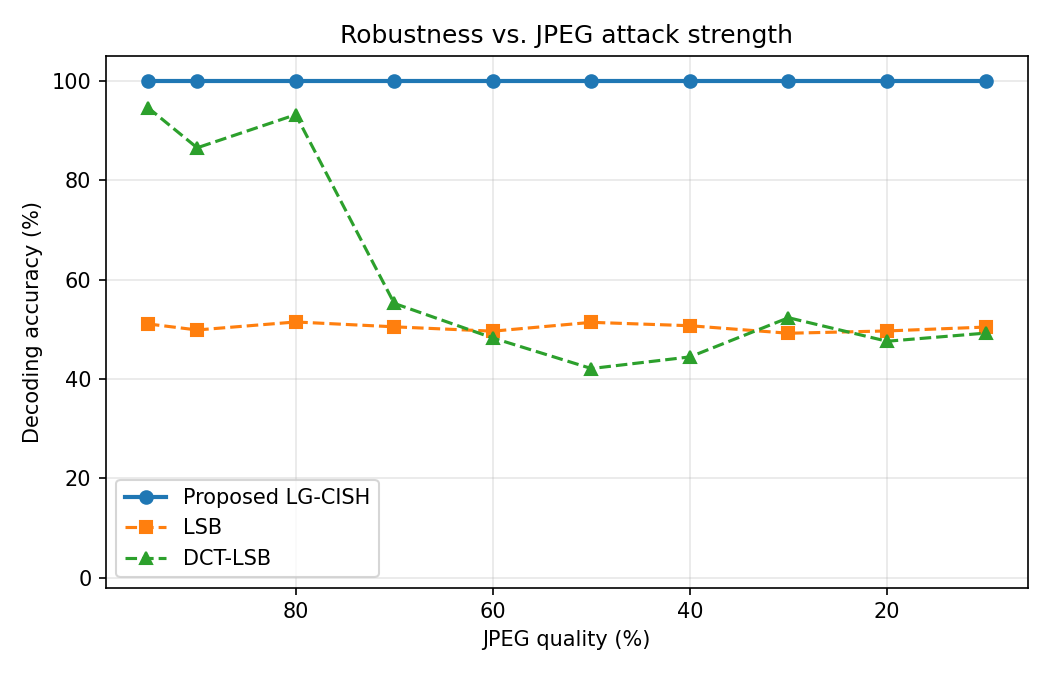
\includegraphics[width=0.86\linewidth]{fig_4_7_robustness_jpeg.png}
\caption{Decoding accuracy vs.\ JPEG quality. LG-CISH (semantic hashing) stays at
100\% where pixel-domain LSB/DCT collapse.}
\label{fig:robcurve}
\end{figure}

\begin{figure}[t]
\centering
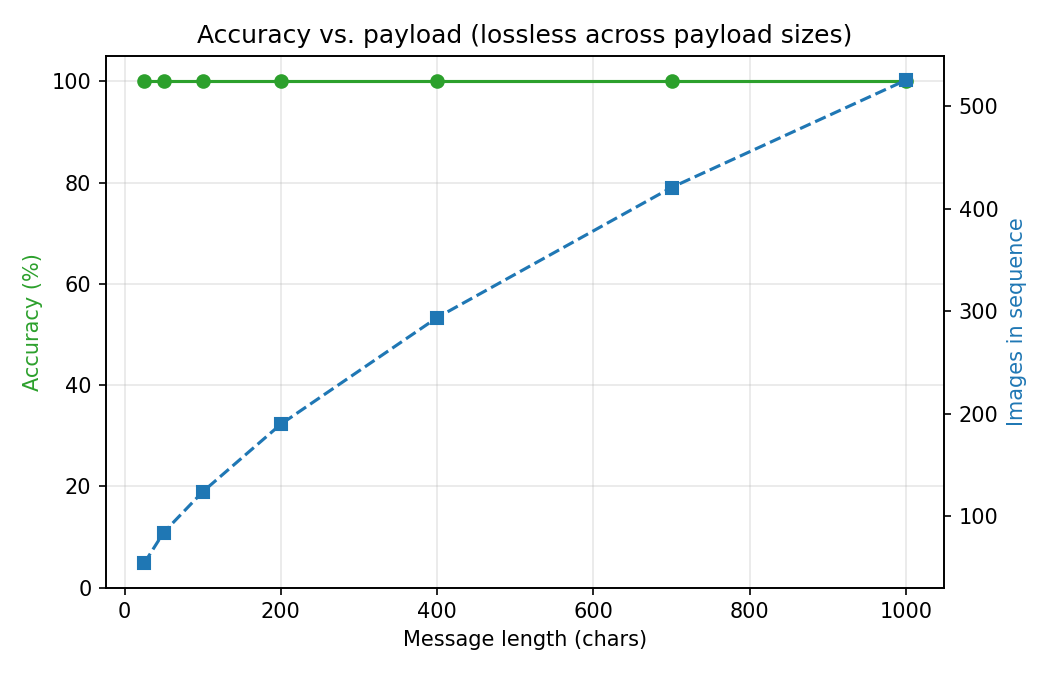
\includegraphics[width=0.86\linewidth]{fig_4_7_accuracy_payload.png}
\caption{Reconstruction accuracy vs.\ payload length. Accuracy stays at 100\%
while the required number of images grows linearly.}
\label{fig:paycurve}
\end{figure}

\begin{figure}[t]
\centering
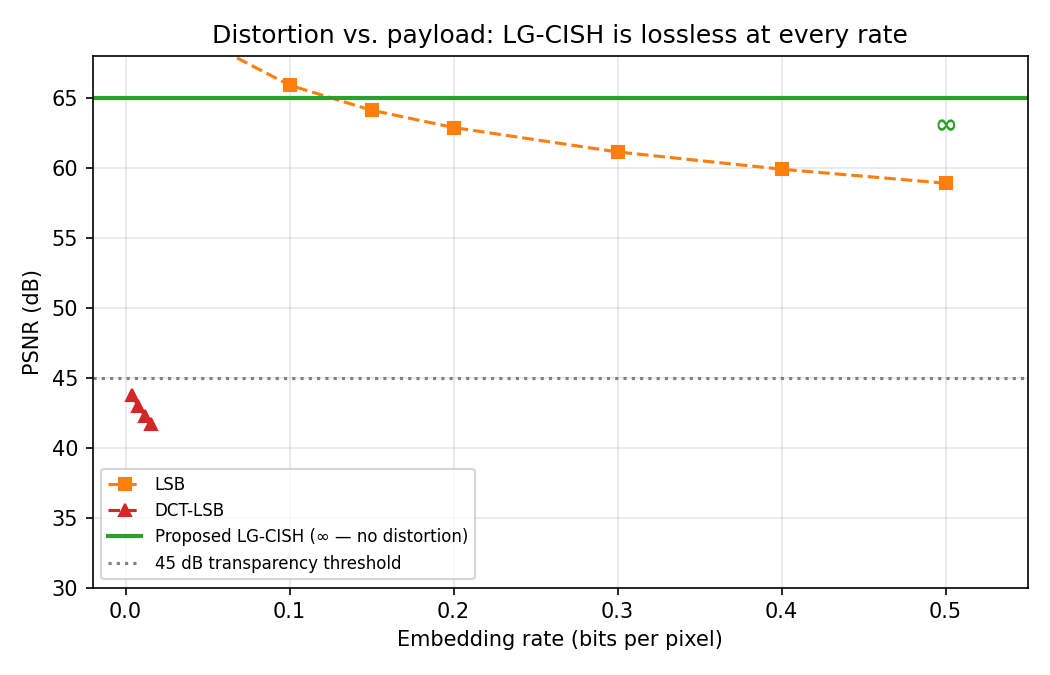
\includegraphics[width=0.86\linewidth]{fig_4_7_psnr_bpp.png}
\caption{Distortion vs.\ embedding rate. Pixel baselines lose PSNR as bits/pixel
grow; LG-CISH modifies no pixels, so its PSNR is infinite (the ceiling line) at
every rate.}
\label{fig:psnrbpp}
\end{figure}

\begin{figure}[t]
\centering
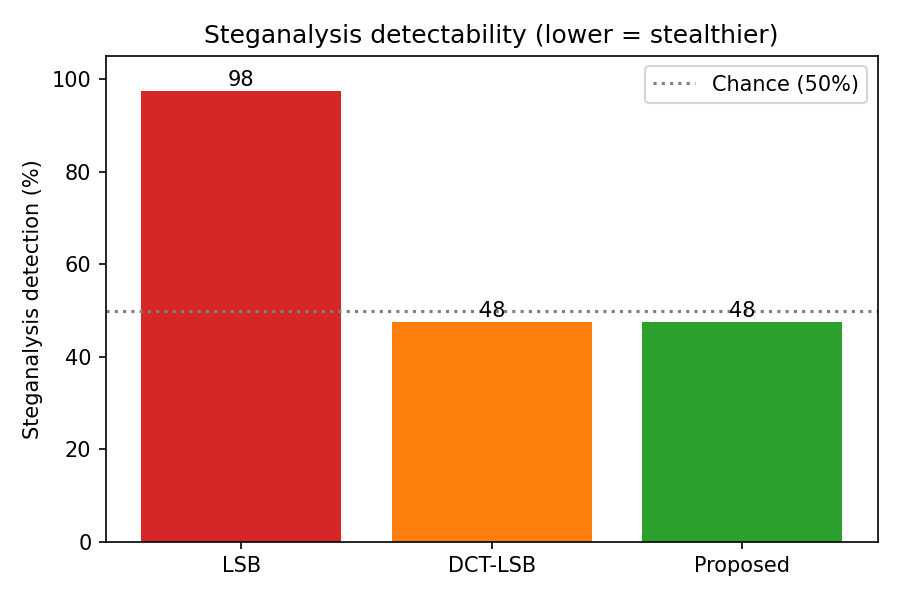
\includegraphics[width=0.7\linewidth]{fig_4_7_detection.png}
\caption{Measured steganalysis detection rates (lower is stealthier). LG-CISH sits
at the 50\% chance line.}
\label{fig:detbar}
\end{figure}

\subsection{Statistical validation}
Over $N{=}50$ independent trials (Table~\ref{tab:stats}) reconstruction accuracy
is $100.00\pm0.00\%$ and BER is $0$, with a stable CLIP margin
$0.3020\pm0.0059$. Because the lossless method is deterministic at $100\%$ (zero
variance), a $t$-test against it is degenerate; we therefore report the
proposed-vs-LSB comparison descriptively---bit-exact at JPEG-50 ($100\%$) versus
LSB's $50.2\pm1.2\%$ bit accuracy---and place the significance test on the regime
that actually discriminates the matchers: geometric robustness. Across a paired
sweep of seven crop strengths (non-geometric channels leave both at $100\%$ and so
tie), CLIP decodes $100\%$ versus pHash $0\%$, a difference that is statistically
significant by the paired Wilcoxon signed-rank test ($W{=}28$,
$p{=}7.8\times10^{-3}$; e.g.\ at Crop-65\%, $100\%$ vs.\ $0\%$). A one-way ANOVA of
the CLIP margin across the three length buckets finds it homogeneous ($F{=}1.99$,
$p{=}0.15$), i.e.\ message length does not affect recovery reliability.

\begin{table}[t]
\centering
\caption{Mean $\pm$ std and 95\% confidence intervals over $N{=}50$ trials (clean channel).}\label{tab:stats}
\begin{tabular}{@{}lcc@{}}
\toprule
Metric & Mean $\pm$ Std & 95\% CI \\
\midrule
Reconstruction accuracy (\%) & $100.00\pm0.00$ & $[100.00,100.00]$ \\
Bit error rate               & $0\pm0$         & $[0,0]$ \\
CLIP margin                  & $0.3020\pm0.0059$ & $[0.3003,0.3037]$ \\
Images per message           & $181.2\pm44.5$  & $[168.5,194.0]$ \\
\bottomrule
\end{tabular}
\end{table}

\begin{table}[t]
\centering
\caption{Significance of CLIP's geometric robustness over the pHash matcher: paired Wilcoxon signed-rank across a crop-strength sweep (proposed-vs-LSB @ JPEG-50 shown descriptively, as the lossless method is deterministic).}\label{tab:signif}
\begin{tabular}{@{}lc@{}}
\toprule
Group / statistic & Accuracy (\%) \\
\midrule
Proposed (CLIP) --- crop-sweep mean & $100.0\pm0.0$ \\
pHash ablation --- crop-sweep mean  & $0.0\pm0.0$ \\
\midrule
Wilcoxon $W$ (paired, 7 crop levels) & $28.0$ \\
$p$-value (one-sided, CLIP $>$ pHash) & $7.8\times10^{-3}\ (<0.05)$ \\
Ref.\ Proposed vs.\ LSB @ JPEG-50 & $100$ vs.\ $50$ (descriptive) \\
\bottomrule
\end{tabular}
\end{table}

% -------------------------------------------------------------------

\ifdefined\LGCISHMAIN\else
\end{document}
\fi
